% it/figures/background/amoc_schematic.tex — versione italiana
\begin{figure}[!ht]
    \centering
    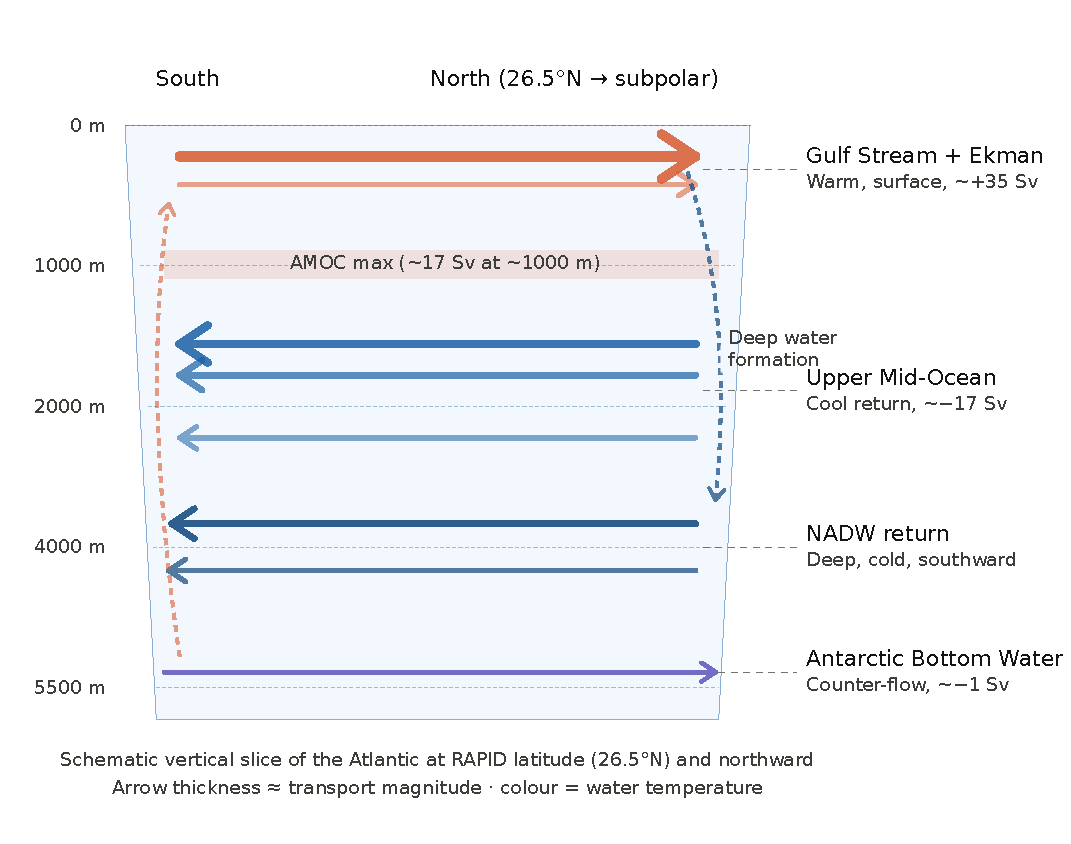
\includegraphics[width=0.9\textwidth]{figures/background/amoc_atlantic_cross_section.pdf}
    \caption[La circolazione di rovesciamento atlantica.]{\textbf{La circolazione di
    rovesciamento atlantica in sezione trasversale.} L'acqua calda superficiale fluisce
    verso nord (arancione), cede calore all'atmosfera nei mari subpolari, diventa densa
    e sprofonda, e ritorna verso sud come una fredda corrente profonda (blu). Il
    rovesciamento verticale è guidato dalle differenze di densità dovute a temperatura
    e salinità. La circolazione non ha alcuna espressione visibile in superficie ---
    l'invisibilità che la tesi si propone di affrontare.}
    \label{fig:amoc-schematic}
\end{figure}
